\section{Problemas NP-Difícil}
Na classe de problemas \textbf{NP-difícil} estão os problemas considerados tão difíceis quanto qualquer outro problema \textbf{NP}. Dizer que um problema é tão difícil quando outro é um tanto subjetivo, mas por definição um problema é tão difícil quanto outro se for possível realizar uma redução polinomial entre eles \cite{HOPCROFT1974}.

Os problemas \textbf{NP-difíceis} não são necessariamente problemas \textbf{NP}, existe uma intersessão entre as duas classes como pode ser visto na figura da página \pageref{intersessao-np-npdificil}.

\begin{figure}
\centering
\label{intersessao-np-npdificil}
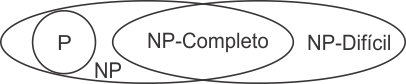
\includegraphics[scale=3]{./figuras/figNP.png}
\caption{Intersessão entre \textbf{NP} e \textbf{NP-difícil} \cite{VIEIRA2001}}
\end{figure}
